\section{Results}

Under the reference configuration, most meta-latents (64.0\%) recur across seeds, suggesting seed reproducibility.
The real seeds' raw agreement is 0.737 while the noise twins' is 0.338 (0.07\% of meta-latents recurring), so excess agreement is 0.400 [0.397, 0.402], and no real or twin meta-latent is dead.
Meanwhile, the main sweep setups score lower, where excess agreement at 2k epochs reaches 0.301 (27B, width 1/32) and 27.8\% of meta-latents recur (27B, width 1/128), while at 4k epochs both measures peak at width 1/32 for 27B, with 0.317 and 29.9\% respectively.
On the 4B 16k parent's meta-SAEs, matching the training steps of 2,000 epochs on a 65k parent results in 33.4\% of meta-latents recurring at width 1/64.

\begin{figure}[t]
  \centering
  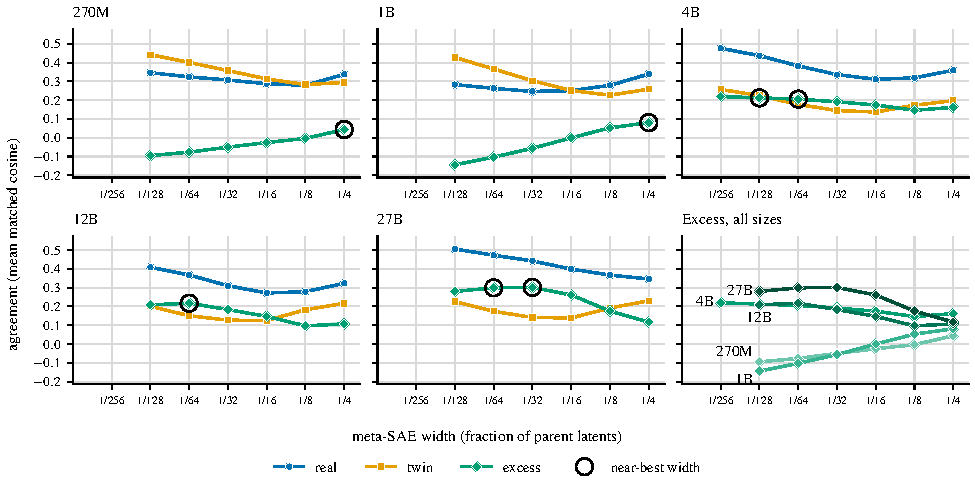
\includegraphics[width=\linewidth]{figures/width.pdf}
  \caption{Real, twin, and excess agreement of the main sweep's meta-SAEs over width at 2,000 epochs. One panel per model size, plus a sixth with all five excess curves. Near-best widths among the six main widths are circled (for 4B, considering 1/256 would shift the near-bests to 1/128 and 1/256). Bands (90\% jackknife intervals over seeds) are all narrower than the markers.}
  \label{fig:width}
\end{figure}

\subsection{Width}

Noise twin raw agreement traces a shallow U over width at every model size (Figure~\ref{fig:width}), bottoming at 1/8 width for Gemma 3 270M and 1B and at 1/16 for sizes 4B and larger.
Real raw agreement is also a shallow U at every size but 27B, where it rises with all narrower widths, and at 1B bottoms out at 1/32 instead of the noise twin's 1/8.

Among the six main widths, 1/128 yields the highest raw real agreement at every size except 1B (where 1/4 is best), but excess agreement reveals a starkly different trend.
Regardless of keeping or dropping dead meta-latents, excess agreement peaks at 1/4 for 270M and 1B and at 1/128, 1/64, and 1/32 for 4B, 12B, and 27B.
Considering excess agreement instead changes the top width for 270M, 27B, and, narrowly, 12B.
Notably, 270M's top width by real raw agreement (1/128) is the worst width by excess agreement ($-$0.095 [$-$0.098, $-$0.093]).

Mean excess interval is negative from 1/8 and smaller for 270M, and from 1/32 and smaller (1/16 after 4k epochs) for 1B.
All widths of both scale sizes show real meta-latents having a greater recurring fraction than their noise counterparts (by 1.4 to 7.2 percentage points, such as 2.5\% vs 0.7\% for 270M's 1/128).

Every size's upturns in raw agreement at 1/4 for both real (except at 27B) and noise twin coincide with a large gap in the real meta-SAEs' explained variance between training and test rows (4.1 to 5.9 times; Appendix~D).
Correspondingly, the split in excess agreement trends between 1B and 4B comes with a jump in dead noise twin meta-latents at 1/4, from 0\% to between 17.1\% and 22.3\%.

\subsection{Model size}

The highest excess agreement seems to increase with model size, from 0.043 at 270M to 0.301 at 27B, though the 4B and 12B tops overlap (Appendix~E) while 270M and 1B's top width is 1/4 but every width from 1/32 to 1/128 at 4B and larger beats 1/4 (top width scores 0.050 to 0.184 more, with intervals above 0).
Live-only excess agreement shows the same ordering.
The jump from 1B to 4B corresponds with lower noise twin agreement at every width (halves for 1/32, from 0.303 to 0.145).
Widths 1/32 to 1/128 at the larger sizes also have 1.9 to 3.3 times the recurring fraction of 1/4 at the same size.
12B and 27B's excess agreements peak at non-end widths (1/64 and 1/32) while 4B peaks at its narrowest (1/256, beating 1/128 by only 0.007 [$-$0.009, 0.024]).

\begin{figure}[t]
  \centering
  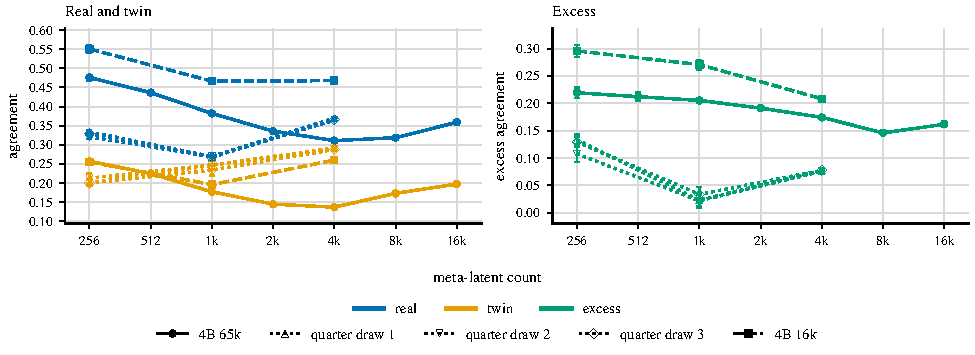
\includegraphics[width=\linewidth]{figures/arms.pdf}
  \caption{At equal steps (26,000), the 4B control meta-SAEs' real, twin, and excess agreement over the number of meta-latents, for meta-SAEs trained on the three quarter draws of the 4B 65k parent's rows and on the 4B 16k parent at widths 1/4, 1/16, and 1/64, and on the 4B 65k parent at 1/4 to 1/256. Error bars are 90\% jackknife intervals over seeds.}
  \label{fig:arms}
\end{figure}

\subsection{What width tracks}

Given equal training steps and the same width or meta-latent count, meta-SAEs trained on the 4B 16k parent score 0.034 to 0.096 higher than those trained on the 4B 65k parent, which themselves score 0.072 to 0.184 higher than those trained on a random quarter of the 4B 65k rows (Figure~\ref{fig:arms}).
It seems that training on fewer rows of the same parent coincides with lower excess agreement at a fixed width or meta-latent count, and that training on a smaller parent can actually raise excess agreement at a fixed count (Appendix~E).
It is also reasonable to say that none of width, meta-latent count, or training row count alone determines excess agreement.

The fifth control, the 270M 16k parent, tests whether a parent's number of latents per hidden dimension explains excess agreement.
It has the same latent count per hidden dimension (25.6) as the 4B 65k parent and a quarter of the 270M 65k parent's 102.4 (Table~\ref{tab:parents}).
Since it also has a quarter of the 270M 65k parent's rows, which by itself lowers excess agreement, only clearly positive excess agreement at narrow widths would support latents per hidden dimension as an explanation.
Given equal training steps, its meta-SAEs show no such gain.
Their excess agreement is 0.049 at width 1/4 (unchanged live-only), $-$0.026 at 1/16 and $-$0.068 at 1/64, each within 0.009 of the 270M 65k parent's at the same width, and only the 1/4 difference excludes 0 (Tables~\ref{tab:app-arms} and~\ref{tab:app-arm-diff}).
At the same meta-latent count, the differences are larger (+0.013 to +0.075), since each partner is a narrower 270M 65k width, where excess agreement is lower.
Thus, latents per hidden dimension alone does not determine excess agreement.

\subsection{Robustness}

\begin{figure}[t]
  \centering
  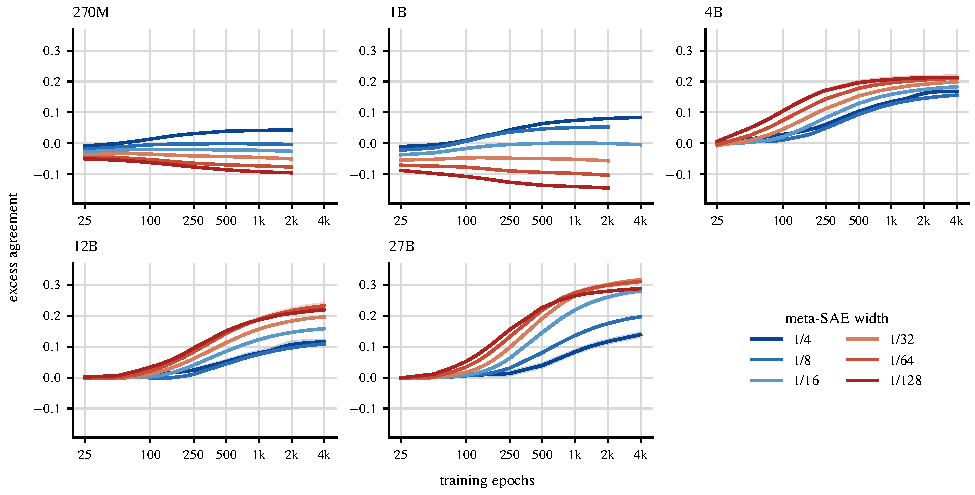
\includegraphics[width=\linewidth]{figures/length.pdf}
  \caption{The six main widths' excess agreement over training epochs (2k or 4k epochs, depending on the training length extension rule), from training snapshots (every 25 epochs up to epoch 250, then every 250 epochs) and the final dictionary, with one panel per model size. Bands are 90\% jackknife intervals over seeds and are mostly narrower than the lines.}
  \label{fig:length}
\end{figure}

\paragraph{Training distance.}
From 4B to 27B, the top and near-best main widths are the same at 2,000 epochs and 4,000 epochs, and the top width's gap above 1/4 moves by at most 0.008.
Even at 4,000 epochs, excess agreement still rising at every 27B width and at 12B widths 1/8 to 1/128 (Figure~\ref{fig:length}) suggests that training had not fully converged.
As for the negative excess for narrow widths on 270M and 1B, overtraining is not to blame since said negative excess appears after just 25 epochs, before 270M's real validation loss bottoms out.
Negative excess agreement on widths 1/64 and 1/128 for 270M also shows in the 1e-3 learning rate check (Appendix~B).
The rate check also shows 27B's narrow widths scoring above 1/4.

\paragraph{Dead latents and the live-only view.}
Dropping dead meta-latents changes no near-best set at any size or length, with or without 1/256.
Dead meta-latents mostly concentrate at width 1/4 for sizes 4B and larger, with the noise twins having more (at 2,000 epochs, 17.1\% to 22.3\% against 1.0\% to 14.5\%), and live-only excess agreement also showing width 1/4 as the worst at both 2,000 and 4,000 epochs.
